\documentclass[a4paper]{article}

\usepackage{fullpage} % Package to use full page
\usepackage{parskip} % Package to tweak paragraph skipping
\usepackage{tikz} % Package for drawing
\usepackage{amsmath}
\usepackage{hyperref}
\usepackage{verbatimbox}
\usepackage{listings}
\usepackage{xcolor}
\usepackage{subfigure}

\definecolor{mygreen}{rgb}{0,0.6,0}
\definecolor{mygray}{rgb}{0.5,0.5,0.5}
\definecolor{mymauve}{rgb}{0.58,0,0.82}
\lstset{ %
  backgroundcolor=\color{white},   % choose the background color
  basicstyle=\footnotesize,        % size of fonts used for the code
  numberstyle=\tiny,
  breaklines=true,                 % automatic line breaking only at whitespace
  captionpos=b,                    % sets the caption-position to bottom
  commentstyle=\color{mygreen},    % comment style
  escapeinside={\%*}{*)},          % if you want to add LaTeX within your code
  keywordstyle=\color{blue},       % keyword style
  stringstyle=\color{mymauve},     % string literal style
}

\title{CSCE 569: Homework 4}
\author{Nick Tyler}
\date{05/04/18}

\begin{document}

\maketitle

\section*{Jacobi Iterative Method}
Similar to the matrix multiplication problem the matrices need to be allocated and copied into the GPU memory. The values which do not change were copied into constant memory, instead of being called in the kernel function call.
\begin{lstlisting}[language=C++]
int size = (sizeof(REAL) * n * m);
REAL *cuda_u;
REAL *cuda_f;
REAL *cuda_uold;
REAL *cuda_resid;
// Copy u to cuda memory
cudaMalloc((void **)&cuda_u, size);
cudaMemcpy(cuda_u, u, size, cudaMemcpyHostToDevice);
cudaMalloc((void **)&cuda_f, size);
cudaMemcpy(cuda_f, f, size, cudaMemcpyHostToDevice);
cudaMalloc((void **)&cuda_uold, size);
cudaMalloc((void **)&cuda_resid, size);
\end{lstlisting}

The kernel function will be called inside the while loop, after the u and uold are swapped. The residual is computed on the GPU and then the matrix is copied back to the host where the error was computed. There were many attempts to compute the error on the GPU but the solutions were either slower or did not return the proper error value to the host.
\begin{lstlisting}[language=C++]
while ((k <= mits) && (error > tol)) {
	error = 0.0;
    /* TODO #3: swap u and uold */
    temp = cuda_u;
    cuda_u = cuda_uold;
    cuda_uold = temp;
    /* TODO #5: launch jacobi_kernel */
    jacobi_kernel <<<dimGrid, dimBlock>>> 
    		(cuda_u, cuda_uold, cuda_resid, cuda_f);
    /* Error check */
    cudaMemcpy(resid, cuda_resid, size, cudaMemcpyDeviceToHost);
    for (i = 1; i < (n - 1); i++)
      for (j = 1; j < (m - 1); j++) {
        error += resid[i * n + j] * resid[i * n + j];
      }
    if (k % 500 == 0) 
    		printf("Finished %ld iteration with error: %g\n", k, error);   		
	error = sqrt(error) / (n * m);
    k = k + 1;
}
\end{lstlisting}
\pagebreak
\section*{Jacobi CUDA Kernel}
Inside the kernel the loops were unrolled similar to the matrix multiplication, using the blockId,blockDim and threadId to get the proper elements of the matrix and computing the residual from those elements. It's important not to go over the bounds of the matrix so if the row and col are on the boundaries, the function returns without computing anything.
\begin{lstlisting}[language=C++]
int row = blockIdx.x * blockDim.x + threadIdx.x;
int col = blockIdx.y * blockDim.y + threadIdx.y;
if (row == 0 || col == 0) return;
if (row >= (c_n - 1) || col >= (c_m - 1)) return;
resid[row*c_n+col] = (c_ax * (uold[(row-1)*c_n+col]
  					+ uold[(row+1)*c_n+col])
  					+ c_ay * (uold[row*c_n+(col-1)]
  					+ uold[row*c_n+(col+1)])
  					+ c_b * uold[row * c_n + col] 
  					- cuda_f[row * c_n + col]) / c_b;
u[row*c_n+col] = uold[row*c_n+col] - c_omega*resid[row*c_n+col];
\end{lstlisting}

\section*{Matrix Multiplication Performance}
The graphs on the following page show the performance of the different matrix multiplication kernels used. The fastest of the implementations in total running time was the shared memory kernel, whereas the slowest was the cublas example. This is very strange since when looking at the detailed performance measurements the cublas was the most efficient. It seems like part of the problem with the cublas kernel is the malloc and free functions for cublas slow down it's implementation. When looking at the performance in detail it is clear to see this:
\begin{lstlisting}[language=bash]
 55.61%  789.60ms         8  98.701ms  17.974us  787.45ms  cudaFree
 40.97%  581.80ms         7  83.114ms  13.747us  579.89ms  cudaMalloc
 \end{lstlisting}

Although the kernel is more complicated the shared memory kernel has a major improvement over the vanilla kernel. If these same ideas were implemented in the jacobi kernel there would be a major improvement in the speed instead of the minor improvement at the moment. However this would also introduce more boundaries into the jacobi calculation making it more difficult to implement than the standard matrix multiplication kernel.
 
\pagebreak
\begin{figure}[h]
\subfigure[Matrix Multiplication]{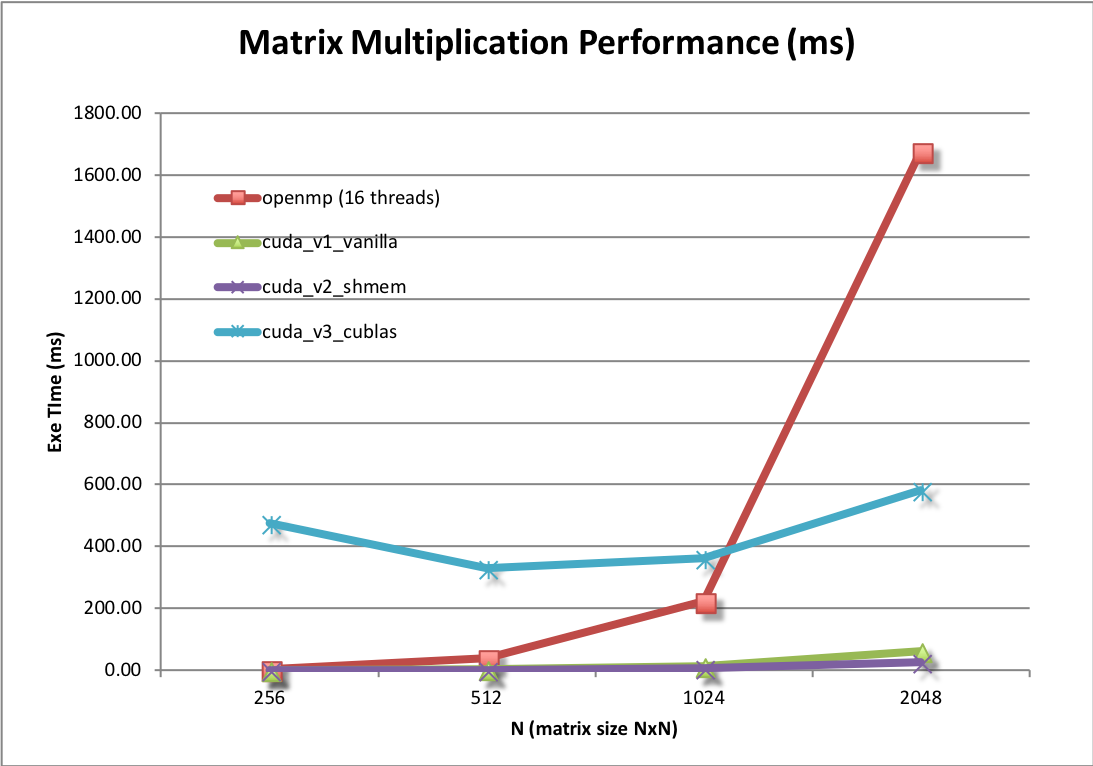
\includegraphics[scale=0.7]{MatMul.png}}
\vfill
\subfigure[Performance]{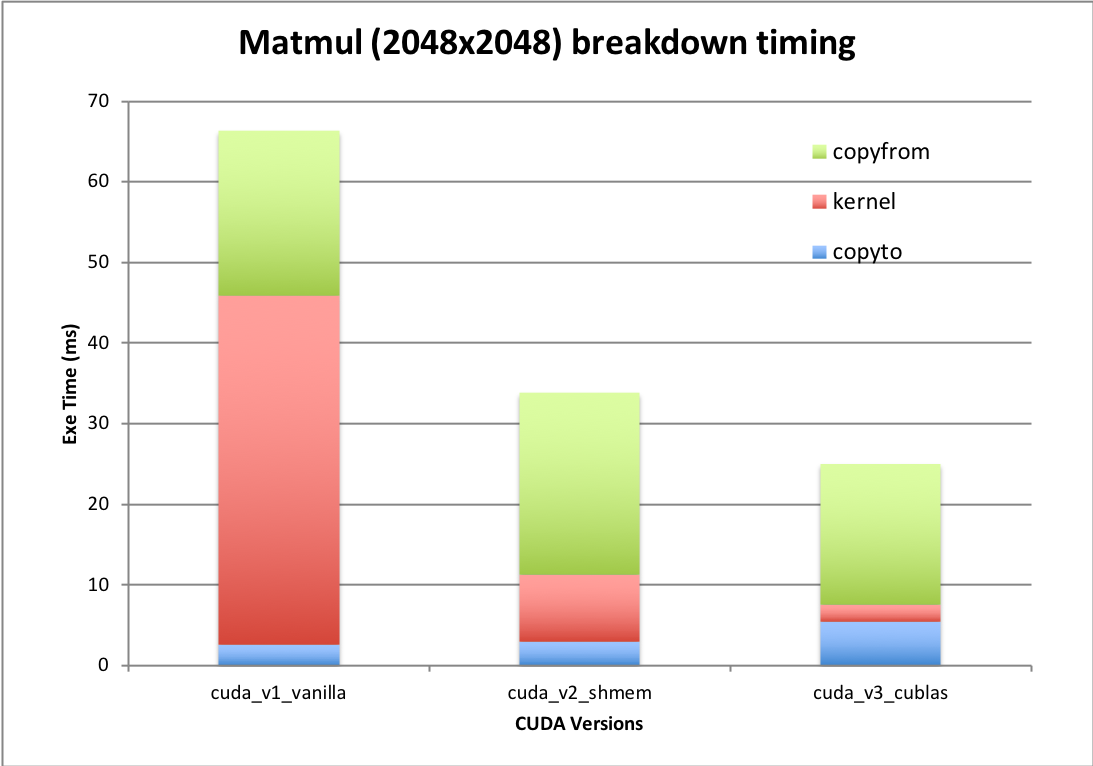
\includegraphics[scale=0.7]{Breakdown.png}}
\caption{Performance Graphs}
\end{figure}

\pagebreak

\end{document}
              
            
